\section{Исследование и построение решения задачи}
\label{sec:Section3} \index{Section3}

\subsection{Сбор данных для дальнейшего тестирования}

В данной работе генерация сигнатуры приложений рассматриваться не будет,
так как все современные приложения используют шифрование, а административные методы,
позволяющие дешифровывать поступающий трафик, остаются за рамками данного исследования.
Однако были выбраны такие протоколы, которые покрывают все основные возможные проблемы,
возникающие при генерации сигнатуры приложений, которые были описаны раннее.

Будут рассматриваться следующие протоколы: HTTP, FTP, DNS, IMAP, SMTP, POP3, BitTorrent \cite{Bittorent}.
HTTP - типичный представитель текстового протокола, который используется не только веб-приложениями,
но и в качестве туннеля.
FTP использует множественное подключение (как минимум двойное), при этом один канал является управляющим,
а через остальные происходит передача данных. DNS является представителем бинарного протокола, использующий UDP.
IMAP, SMTP, POP3 - стандартные почтовые протоколы, сообщения у них обычно короткие.
BitTorrent - P2P протокол для кооперативного обмена файлами.

Исследуемый сетевой трафик снимался с кампусной сети ИСП РАН. Затем с помощью Wireshark \cite{Wireshark}
этот трафик был разбит по протоколам и результатом его работы были .pcap - файлы,
которые содержали в себе сессии определенного протокола, захваченные в течении исследуемого сетевого взаимодействия.

\begin{figure}[H]
    \begin{center}
        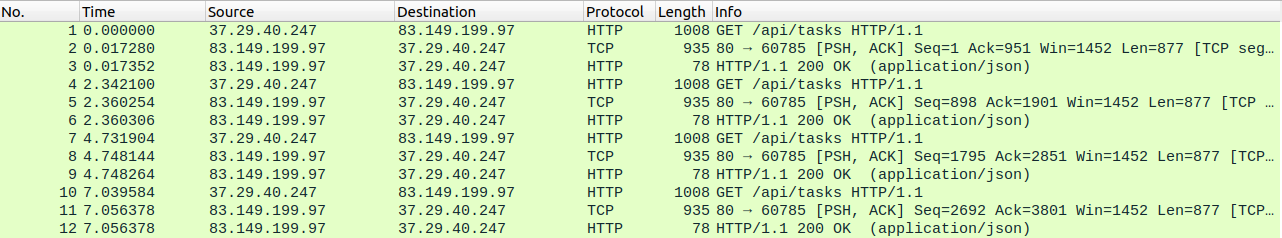
\includegraphics[width =\textwidth]{Wireshark.png}
        \caption{Пример работы Wireshark.}
    \end{center}
\end{figure}

\subsection{Выбор алгоритма для автоматической генерации сигнатур}
Алгоритм LASER достаточно простой, так как основан на LCS, поэтому отлично подходит для первичной разработки сопутствующей инфраструктуры,
а также для различных модификаций, чтобы оценить поведения сигнатур в сетевом трафике при разных условиях.


Система AutoSig ввела дерево подстрок.
Данная структура хороша тем, что увеличивает мощность получаемых сигнатур,
это позволяет выделить несколько последовательностей подстрок, которые могут охватить те ситуация, когда
приложение имеет сильно разные потоки (например, поток управления и поток данных в FTP).
Однако в том в виде, в котором это дерево преставлено в работе, получается сильно избыточный результат.
Если узел является сигнатурным и не листом, то по свойству этого узла его набор потоков является строгим надмножеством
наборов потоков любых других сигнатурных узлов, находящихся в его поддереве (например, листы, которые всегда являются сигнатурными),
таким образом, любые пути из сигнатурных узлов поддерева являются избыточнымы, так как если нашлась последовательность подстрок
соответствующая сигнатурному узлу из рассматриваемого поддерева, то найдётся в потоке и последовательность подстрок, соответствующая рассматриваемому узлу.
При этом специфичность нашей сигнатуры за счёт этих сигнатурных узлов не увеличивается,
так как для совпадения со сигнатурой достаточно совпадания последовательности подстрок, соответствующей нашему узлу, которая уже включена в другие.
А значит поддерево можно удалить. Однако если не выполняется строгость надмножества, то последовательности строк
поддерева не будут включаться друг в друга, а полнота покрытия потоков сохраниться,
при этом вырастит специфичность (чем длиннее последовательность подстрок, тем специфичнее сигнатура).
Именно поэтому при таком условии узел не становится сигнатурным.

SigBox должен быть не чувствителен к шумам, поэтому можно попробовать выделить сигнатуру на не размечанном трафике.

\subsection{Реализация алгоритма LASER}



\newpage
